% \documentclass[tikz, convert={density=300,size=1080x800,outext=out_pic.png}]{standalone}
\documentclass[tikz]{standalone}
%\documentclass{article}
\usetikzlibrary{decorations.fractals}
\usetikzlibrary{lindenmayersystems}

\begin{document}
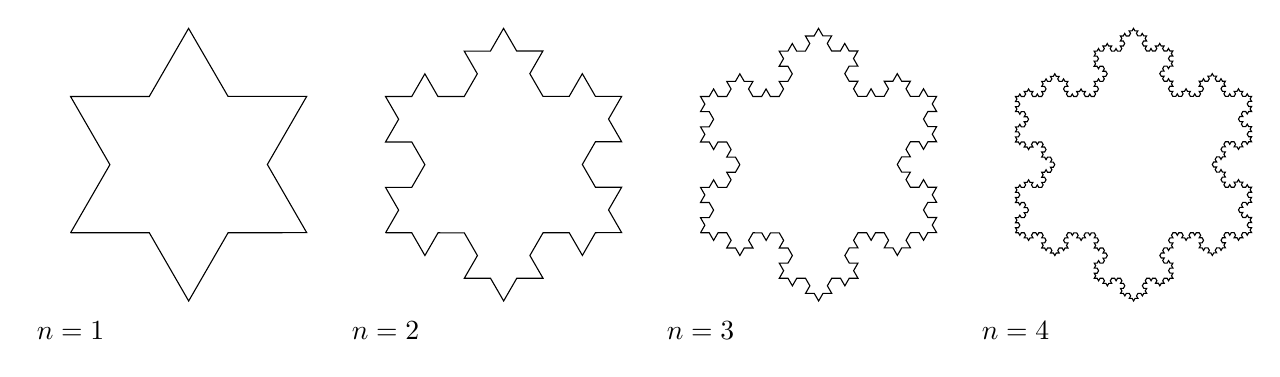
\begin{tikzpicture}[decoration=Koch snowflake]
\draw decorate {(0,1) -- ++(60:3)  -- ++(300:3) -- ++(180:3)} node[below=1cm](init){$n=1$};
\draw decorate { decorate {(4,1) -- ++(60:3)  -- ++(300:3) -- ++(180:3)}} node[below=1cm](two){$n=2$};
\draw decorate{decorate { decorate {(8,1) -- ++(60:3)  -- ++(300:3) -- ++(180:3)}}} node[below=1cm](nthree){$n=3$};
\draw decorate {decorate{decorate { decorate {(12,1) -- ++(60:3)  -- ++(300:3) -- ++(180:3)}}}} node[below=1cm](nfour){$n=4$};
\end{tikzpicture}
% Use the following for live preview
% latexmk -pdf -pvc -shell-escape --interaction=nonstopmode
% convert -resize 1200x1200 -density 7200 -quality 75 file.tex file.png
% convert -resize 1200x1200 -density 7200 file.tex file.svg
\end{document}

